\documentclass[12pt,a4paper,onecolumn]{article}
\usepackage[utf8]{inputenc}
\usepackage{amsmath}
\usepackage{amsfonts}
\usepackage{amssymb}
\usepackage{graphicx}
\usepackage[margin=1in]{geometry}
\usepackage{mathpazo}
\usepackage{float}
\usepackage{color}
\usepackage{hyperref}
\hypersetup{
    colorlinks=true,
    linkcolor=black,
    urlcolor=red,
    linktoc=all
}
\usepackage[toc,page]{appendix}

\addtocontents{toc}{\protect\hypertarget{toc}{}}
\usepackage{algorithmic}
\usepackage{newunicodechar}
\newunicodechar{fi}{fi}
\newunicodechar{fl}{fl}

\author{Anya Chaturvedi \\ Sagar Sahni \and K. R. Prajwal \\ Ketaki Vaidya  }
\title{%
  The Capacitated K-Center Problem\\
  \large Summer Internship Report 
  ($9^{th} May-8^{th} July$)}
 \date{}
\begin{document}
\begin{titlepage}

\newcommand{\HRule}{\rule{\linewidth}{0.5mm}} 

\center 

%\textsc{\LARGE Capacitated K-Center Problem}\\[1.5cm] % Name of your university/college
\textsc{\Large Summer Internship}\\[0.5cm] % Major heading such as course name
\textsc{\large Indian Institute of Technology, Delhi}\\[0.5cm] % Minor heading such as course title



\HRule \\[0.4cm]
{ \huge \bfseries Capacitated K-Center Problem}\\[0.4cm] % Title of your document
\HRule \\[1.5cm]
 
%----------------------------------------------------------------------------------------
%   AUTHOR SECTION
%----------------------------------------------------------------------------------------

\includegraphics[scale=0.06]{iitd_logo.png}\\[1cm] % Include a department/university logo - this will require the graphicx package



{\large May $9^{th}$ - July $8^{th}$}\\[9cm] % Date, change the \today to a set date if you want to be precise

%----------------------------------------------------------------------------------------
%   LOGO SECTION
%----------------------------------------------------------------------------------------


 \begin{minipage}{0.4\textwidth}
\begin{flushleft} \large
\emph{\\Authors:}\\
Anya Chaturvedi\\
K.R. Prajwal\\
Sagar Sahni\\
Ketaki Vaidya
 % Your name
\end{flushleft}
\end{minipage}
~
\begin{minipage}{0.4\textwidth}
\begin{flushright} \large
\emph{Supervisor:} \\
Dr. Naveen Garg \\
Professor\\
Dept. of CSE\\
IIT Delhi % Supervisor's Name
\end{flushright}
\end{minipage}\\[2cm]
%----------------------------------------------------------------------------------------

\vfill % Fill the rest of the page with whitespace

\end{titlepage}
\maketitle
\tableofcontents
%\section[Abstract]{Abstract \begin{flushright}\hyperlink{toc}{TOC}\end{flushright}}
\section{Abstract}
The capacitated $K$-center problem is basically a facility location problem, where one is asked to assign $K$ points to $K$ facilities in a given distance metric. In doing this we minimize
the maximum distance from a vertex to the facility to which it is assigned while keeping in mind that each facility may be assigned at most $L$ vertices including itself. This problem is known to be NP-hard.

We show our attempts at solving this problem, counter examples as learnt by us and a few basic implementations of the same. Starting by a more formal description of our problem, we describe the flow method which helps us verify a solution to the problem. Next, we implemented the integer program and a partially correct local search algorithm. In implementing the above programs we have used three ways for making the input graphs. One is a random graph, second a more clustered form i.e. a star graph and the last one is generated by taking points in a unit square. Other than this we have included a few observations which may not be much conclusive but are our attempts on solving the problem during the summer.
\section{A Look at the Problem}
The problem taken up by us is actually a generalization of the $K$-center problem which we will explain here. 
\subsection{The $K$-Center Problem}
Given n vertices with specified distances, one wants to build $K$ facilities at different vertices such that each vertex has access to a facility and minimize the maximum distance between the vertex and the corresponding facility. This problem is NP-hard. An approximation algorithm with a factor of $\eta$ ,for a minimization problem,is a polynomial time algorithm that guarantees a solution with cost at most $\eta$ times the cost of an optimal solution. For the basic $K$-center, methods have been presented for obtaining an approximation factor of 2. Given a complete undirected graph G = (V, E) with distances $d(v_i, v_j) \in N$ satisfying the triangle inequality, we have to find a subset $S \subseteq V$ such that $|S| = k$ and covering all $V$.\\\\
 \textbf{Input:}\\1. The vertices must be in a metric space, or in other words IN a complete graph that satisfies the triangle inequality.\\2. An upper bound on the number of centers K.\\\\
\textbf{Formal Definition:}\\
$$\min_{S \subseteq V}\max_{v \in V}\min_{s \in S}d(v,s)$$
where d is the distance function.

This is much similar to the problem of placing k disks such that all points are covered in the set V and thus finding the minimising the maximum radius for the disks.
%\begin{center}

%\begin{figure}[h]
 % \includegraphics[scale=0.5]{kcenter.png}
  %\caption{HELLO}
  %\label{fig:intro}
%\end{figure}
%\end{center}
\subsection{The Capacitated K-Center}
The capacitated K-center problem is nothing but a generalization of the K-center problem. We have to
output a set of at most K centers,as well as an assignment of vertices to centers. No more than L vertices may be assigned to a single center. Under these constraints,we
wish to minimize the maximum distance between a vertex u and its assigned center
$\varphi$(u). \\\\
\textbf{Input:}\\1. The vertices must be in a metric space, or in other words a complete graph that satisfies the triangle inequality.\\2. An
upper bound on the number of centers, K.\\3. A maximum capacity for each center, L.\\\\
\textbf{Formal Definition:}\\
$$ \min_{S \subseteq V}\max_{u \in V}d(u,\varphi(u)) $$such that,   $$|\{u|\varphi(u) = v\}|\leq L \forall v \in S,$$\\where,   $$\varphi : V \rightarrow S.$$\\
The first polynomial time approximation
algorithm for this problem was with an approximation factor of 10. Later a 6-approximation was found which is the best up till date while a 5-approximation works when we can assign multiple centers at a single vertex without including the vertex in L.

Initially we went through the 2.6 and 9.3 sections of Williamson Schmoy which solve the problem of finding the min degree spanning tree problem which is also NP-hard and got to know of methods like local search used to create approximation algorithms.

Certifying a graph for an algorithm not only has to ensure that we can show whether a solution is possible for G or not it also involves showing that if a solution is not possible in G then it is not even possible in $G^2,G^3\ldots$
\section{Checking the Feasibility of the Input Graph}
We say that, if we solve the capacitated K-center problem then it will be equivalent to getting the minimum value of W for which G(W) has a capacitated dominating set of size k, where G(W) refers to the graph having all edges with edge weight less than or equal to W.

We can easily set up such an equivalence if we slightly modify our problem. Given a graph $G = (V,E)$ and a capacity function $c : V \rightarrow N$ and $S \subseteq V$ is a capacitated dominating set if there exists a mapping $f : V \rightarrow S$ (domination mapping) such that:\begin{enumerate}

\item $\forall v \in V ,\forall s \in S,f(v) = s \Longrightarrow (v,s) \in E$\\ \item $\forall s \in S,| \{ v \in V \backslash S | f(v) = s \} | \leq c(s)$
\end{enumerate}In the new version of the k-center problem, the goal is to get a set S of k vertices and an assignment $h : V \backslash S \rightarrow S$ of every vertex (in $V \backslash S$) to an open center such that the longest distance between a vertex and a center it is assigned to is minimum and no facility is assigned more vertices than its capacity. Note that, the assignment is not for all vertices in V . We are making the assumption that every center serves itself and the capacity (L(v)) of a vertex $v \in V$ is the maximum number of clients it can serve (excluding itself). 

Now we can say that, solving the capacitated k-center problem is equivalent to getting the minimum value of W for which G(W) has a capacitated dominating set of size k. 
$S \subseteq V$ is an optimal solution to the capacitated K-center problem if and only if w(S) is the minimum value of W for which the graph G(W) has a capacitated dominating set of size k.
It is also easy to verify that a capacitated dominating set of size k in $G(w(S))^i$, for some i and some optimal solution S, forms an i-approximation for the k-center problem.

But the capacitated dominating set problem is an NP-complete problem. So, we cannot get a capacitated dominating set of size k in polynomial time, unless $P = NP$ Similar to the uncapacitated version the capacitated version too is hard to approximate within a factor of 2.
\subsection{Verification using a Network Flow }
Given a graph $G = (V,E)$ and a capacity function $c : V \rightarrow N$, checking whether $S \in V$ is a capacitated dominating set can be viewed as a network problem. Construct a directed graph $G_S = (V_S,E_S)$ as follows:\begin{enumerate} 
\item $V_S = V \cup \{s,t\}$
\item $E_S = \{(s,v_i) | v_i \in V \backslash S \} \cup \{(s_i,t) | s_i \in S \}\cup \{(v_i,s_i) | v_i \in V \backslash S \wedge s_i \in S \wedge (v_i,s_i) \in E \}$\end{enumerate} Let $c_S : E_S \rightarrow N$ be the capacity function such that, $$c_S(e_{uv}) =\left\{ \begin{array}{cc}(c(u),  &  v = t \\\\ 1, & otherwise \end{array}\right.$$
In the final graph $G_S$ we add two more vertices s (source) and t (sink) to the vertex set of G. We add directed edges from s to all vertices in $V \backslash S$, from each vertex in $V \backslash S$ to its neighbours in S and each vertex in S to t. We take the capacity function to be equal to the capacity of the source vertex for edges incident on t and to be equal to 1 for every other edge in $E_S$. \\
The flow network as described has been shown in the figure:
\begin{flushleft}
 \begin{figure}[H]
 \begin{center}
 \includegraphics[scale=0.55]{diag2.jpg}
 \end{center}
  \caption{The flow network}
  \label{Figure 1}
\end{figure}
\end{flushleft}
  Now it is easy to verify that, S is a capacitated dominating set in G if and only if $G_S$ has a maximum coverage of $|V \backslash S|$ from s to t equal to the total vertices in the graph. 

\section{The Integer Program}
Linear programming is a mathematical technique for maximizing or minimizing a linear function of several variables such as output or cost. The decision variables with respect to which the optimum is obtained can come out to be fractional or any real number. An integer programming problem is a mathematical optimization or feasibility program in which
some or all of the variables are restricted to be integers which is the major difference it has from linear programming. Ours is a problem where we
wish to minimize the maximum distance between a vertex u and its assigned center thus our integer program is framed as:
\\




\textbf{Objective Function:}\\
\hspace{15mm} $$z=\sum_{i=1}^{N}cen[i]$$
\\
\textbf{Variables:}\begin{enumerate}
\item \textit{\textbf{cen}} - an integer dictionary which specifies the centers among the vertices
where if $cen[i]=1$ then the $i^{th}$ index vertex is taken to be a center otherwise not.\item \textit{\textbf{assignments}} - dictionary $assignments[i][j]=1$ will represent that the $j^th$ index vertex is assigned to the center created at the $i^th$ index vertex, we initialize it with the adjacency matrix
\item \textit{\textbf{N}} - represents the total number of vertices
\item \textit{\textbf{adj}} - a dictionary which stores the adjacency matrix of the graph 
\end{enumerate}
\textbf{Constraints:}
\begin{enumerate}
\item $\forall i \sum_{j=1}^{N}assignments[i][j]\leq L*cen[i]$\\\hspace{1cm}\ldots makes sure no more than L vertices are assigned to a center
\item $\forall j \sum_{i=1}^{N}assignments[i][j] = 1$\\\hspace{1cm}\ldots a vertex can be assigned only to a single center
\item $\forall i \, \forall j \, assignments[i][j] \leq cen[i]$\\\hspace{1cm}\ldots a vertex can only be assigned to a second vertex if the second vertex is a center
\item $\forall i , \forall j \, assignments[i][j] \leq adj[i][j]$\\\hspace{1cm}\ldots 
assignment of vertices can only be done if the edge is present in the original graph

\end{enumerate}

You can refer to the code in Appendix A.

\section{Local Search Algorithm}
Local search can be used on problems that can be formulated as finding a solution maximizing a criterion among a number of candidate solutions.
A local search algorithm starts from a candidate solution and then iteratively moves to a neighbour solution. We move from solution to solution in the space of candidate solutions (the search space) by applying local changes, until a solution optimal is found.
We have used a local search algorithm which was formed by Aounon. It doesnt work on a set of graphs but we get the solution for some general graphs we tested on.

Here, we start with a set S of random k vertices in graph G . Let S be the set of all k vertex sets which are formed by replacing one vertex in S by a vertex in V (one-swap vertex sets). We look for the set in S which maximizes the number of dominated vertices. If the optimum set dominates more vertices than S then we set S to that set and continue the process till we have reached a local optima. We do the assignments through a network flow graph.\\\\\\
\textbf{Algorithm:}
\begin{algorithmic}[1]
\STATE $S \leftarrow {v1, v2,…., vk}$
\STATE $S' \leftarrow {one-swap\: vertex\: sets\: of\: S}$
\WHILE {$MaxFlow(G_{V_{max}}, c_{V_{max}}) > MaxFlow(G_S,c_S)$}
\STATE $S \leftarrow V_{max}$
\STATE $S' \leftarrow {one-swap vertex sets of S}$
\STATE $V_{max} \leftarrow argmax _{V \in S} MaxFlow(G_V , c_V )$
\ENDWHILE 
\IF{$MaxFlow(G_S , c_S) = n - k$}
\FORALL {$v \in V$}
\IF{$f_{max}(v,s)=1$}
\STATE $h(v) = s$
\ENDIF
\ENDFOR
\RETURN $S, h$
\ENDIF
\end{algorithmic}


You can refer to the code in Appendix B.






\section{Graph Generation}
\subsection{Random Graph}
For testing the implemented algorithms on random graphs, SNAP, a Python based system developed by Stanford University was used which takes the number of nodes and edges as input and gives a random subgraph of a data set and represent it as an adjacency matrix, ready to be fed into the LP and local search algorithm.

You can refer to the code in Appendix C.

\subsection{Star Graph}
In an attempt to try our programs on a more clustered data set, this program was implemented to create sparsely-connected star graphs, with edges chosen to be added with a probability p.

You can refer to the code in Appendix D.

\subsection{Unit Square}
On discussing our above mentioned methods with Sir he suggested another way for making the input graphs which he felt might give us better  results for further analysis. 
The method proceeds by taking N random points in a unit square.
Calculate the edge weight between all possible pairs of these $N$ points by using different $L^p$ norms, for $p \geq 1$.
Choose a $W$, to denote the maximum edge weight allowed in a particular graph which reduces the edges in the otherwise obtained complete graph. 
Build the graph, with the $N$ random points as nodes and add edges $(a,b)$ if distance between $(a,b)$ is $\leq W$, for all $a,b$ $\in$ $N$. 
Use this graph to obtain the optimal $K$ using a capacity, which we have taken as $L = N/10$.
Use the same graph to check if the randomized local search algorithm yields the optimal solution with the above obtained $K$ and $L$.


Even though this did not strike at first on why this will be in any manner be different than using random graphs, still we decided to proceed with the implementation. During our visualization of the graphs created, we saw that this method gave us a very large variety of graphs, in the sense that the graphs had local clusters, articulation points, isolated vertices, cliques and a wide variation in the degrees of the nodes.

You can refer to the code in Appendix E.
\section{Observations made}
This section is a collection of all our trials and errors during our exploration of this topic along with few of the concepts learnt which provide the base for these trials.
\subsection{Lower Bound on K}
Lets say we make disjoint set of partitions of our input graph nodes such that each partition has two types of vertices. Inner and boundary, the inner vertices are the ones which have no edges outside its partition, while the boundary vertices are vertices which do have edges to other partitions. Let the $i^{th}$ partition be represented by its inner vertices $C_i$ and its boundary vertices as $B(C_i)$.

Since we know K vertices can cover up to L vertices so the max vertices than can be covered is $V = K*L$. Hence the minimum $K$ required to cover $V$ vertices is $\lceil V/L\rceil$. This is a naive lower bound on $K$. But using this concept, we can get a better lower bound. 

Here, in the partitioning as described above, for the vertices other than the boundary vertices we can say that they can only be covered by vertices of their own partition thus we need to open centers in the partition itself for such vertices. Thus, if we say there are $p$ partitions then $\sum_{i=1}^{p}\lceil (C_i-B(C_i))/L\rceil$ vertices are required atleast to cover the graph and hence this comes to be a lower bound. \\\\The above bound has been presented in a research paper already. We observed that, the above mentioned paper is not involving the boundary vertices in formulating a lower bound. So, we toyed for some time with ideas on involving the boundary vertices. We thought using the residual capacity, i.e. $\lceil (C_i-B(C_i))/L\rceil*L-(C_i-B(C_i))$ we may be able to cover some or even all of the boundary vertices. Through this we can decide opening more centers or shifting the centers so as to cover more boundary vertices. But all of this depends upon the connectivity of the particular graph and what kind of partition we take which did not look promising after a point of time either.\\ Later when Jatin and Aounon started thinking towards this way we again applied our thinking on the same.

Lets say we partition the graph into sets of nodes $C_i \: 1 \leq i \leq N$:

\begin{flushright}
\begin{figure}[H]
\includegraphics[scale=0.2]{diag7.jpg}
\caption{Partitioning the Vertex Set}
\end{figure}
\end{flushright}

As discussed before, the minimum number of centers we need to place inside the partition $C_i$ is $\lceil ((C_i-B(C_i))/L) \rceil$. The residual capacity, which can cover boundary vertices as mentioned above is,$\lceil (C_i-B(C_i))/L\rceil*L-(C_i-B(C_i))$ , can be used to cover the boundary vertices. 
\\\\
To do this, a flow network is created:

\begin{center}
\begin{figure}[H]
\includegraphics[scale=0.55]{diag1.jpg}
\caption{$Z=\lceil (C_i-B(C_i))/L\rceil*L-(C_i-B(C_i))$}
\end{figure}
\end{center}
Here $Z$ refers to the remaining capacity of the centers as put in the inner vertices i.e $\lceil (C_i-B(C_i))/L\rceil*L-(C_i-B(C_i))$.
Now there are two cases:
\begin{itemize}
\item If we are not able to find a flow to cover all the boundary vertices within a distance of 2 with the residual capacities, then there exist a set of partitions $P_1, P_2,\ldots P_i$ and $B(P_1), B(P_2),\ldots B(P_i)$ for which Hall’s theorem does not hold i.e.: 
 $$|B|> {\sum_{i=1}^{N}\lceil (P_i-B(P_i))/L\rceil*L-(P_i-B(P_i))}$$
which after rearrangement becomes:\\
$$\lceil (\sum_{i=1}^{N}P_i)/L \rceil > \sum_{i=1}^{N} \lceil P_i/L \rceil   $$
This, in turn, means we can merge the above set of partitions to get a better lower bound. The boundary vertices will always be in the interior of the new set of partitions, because if they were not then it can be covered by a residual capacity, a contradiction.



\item If the flow exists, this is where we are stuck again. We do not know if there is such a set of centers we can choose such that we can make use of all the necessary residual capacity which is actually taken into account by the flow network. 
Our attempt to resolve this:

\begin{flushleft}
\begin{figure}[H]
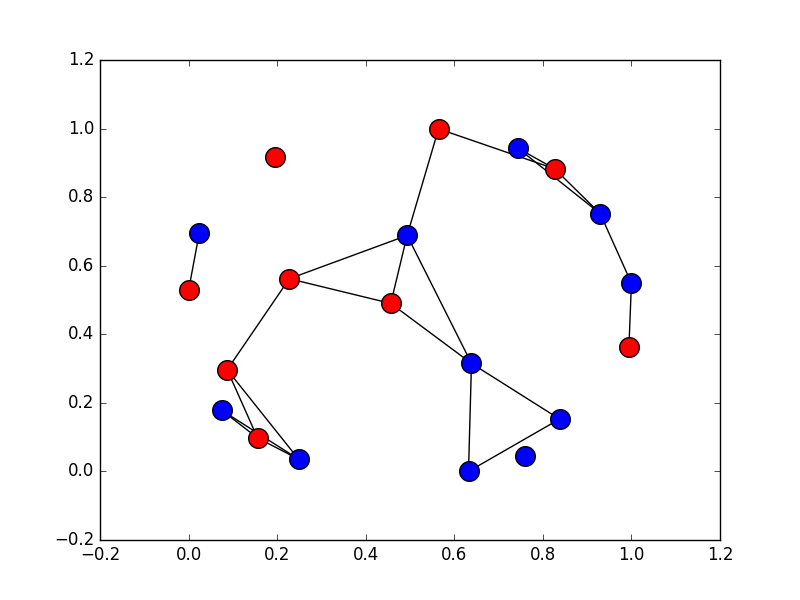
\includegraphics[scale=0.8]{anya.jpg}
  
  \caption{Reassignment of Centers}
\end{figure}
\end{flushleft}

We define
\begin{itemize}


\item Node type: $a$ : A center which does not have edge to any boundary vertex.
\item Node type: $q$ : An interior non - center, which is a client of $a$ and adjacent to a boundary vertex. We will call it the semi boundary vertex. 
\end{itemize} 
We observe that if we make as many semi-boundary centers as possible, such that they cover maximum number of boundary vertices, by shifting the centers located at $a$ to $q$ then we can come to a conclusion. 
If we make the semi-boundary vertex $b$ as a center, then it will cover all the clients that have been covered by its respective center $a$, but now the minimum maximum distance would be at most 4*OPT. Also, we would need to shift to such a set of semi-boundary vertices that maximises the number of distinct boundary vertices getting covered. 

So, we make a flow network:

\begin{flushleft}
\begin{figure}[H]
\includegraphics[scale=0.6]{diag3(2).jpg}
\caption{Flow to exchange Semi-boundary vertices with Existing Centers}
\end{figure}

\end{flushleft}
But we cannot make greedy moves and just move to the semi-boundary vertices with maximum boundary neighbors, as it is very necessary to make sure these boundary neighbours are distinct. To ensure this, we modify the above flow network:
\begin{center}
\begin{figure}[H]
\includegraphics[scale=0.4]{diag4.jpg}
\caption{New Flow Method}
\end{figure}
We keep the capacity of all edges in this flow network as 1 but modify the edge weights of edge weights between B,Q and A to keep a check. Between A and Q, $e_1$ the remaining capacity of $q_i$ which is -- $L-$the number of non centers transferred to it through $a_i$ is taken as the edge weight between $q_i$ and $a_i$. While the edge weight between B and Q, $e_2$ is equal to the inverse of the number of boundary vertices that the corresponding q will cover if selected. 
\begin{figure}[H]
\includegraphics[scale=0.4]{diag6.jpg}
\caption{Case of 2 Available Paths}
\end{figure}
\end{center}
In a case as shown above in the figure if capacity permits, we will choose $e_2 = 1/8$ as it is covering 7 other boundary vertices except the one in the selected augmented path. Also we will have to make changes to the edge weights like converting 1/4 to zero and the corresponding edges of the same semi boundary vertex involved to 1/3 and the semi-boundary to corresponding center as 3. If later 1/8 weight wedge is not a part of the max flow then we simply revert back to the original weights.\\
But we realised that this problem of covering maximum number of boundary vertices is a problem reducible to the max-coverage problem, which is NP-hard. Hence the problem we are trying to solve is indeed NP-hard. The comparison is made by taking the nodes inside the partition as the subsets and the universe outside. 
\begin{center}
\begin{figure}[H]
\includegraphics[scale=0.6]{diag5.jpg}
\caption{Max-Coverage Problem}
\end{figure}
\end{center}
If there is a way where we can get minimum subsets to cover all of the universe then it is the same solution which is not possible.

 However, we still feel that this idea of shifting centers to semi-boundary vertices could lead to some result. 
\end{itemize}
\subsection{Independent Trial}
\begin{itemize}
\item In our attempt we start by applying the 2-approximation K-center algorithm on the given graph. We then tried to apply what we had learnt by reading the OPT + 1 local search algorithm of the min-degree spanning tree from section 2.6 of Williamson \& Schmoy. Effectively,if possible we transferred the load from the highest capacity nodes to lower ones through a contiguous sequence of edge assignment swaps until we reach a vertex with lower capacity as visible in the figure. \\
\begin{figure}[H]
\begin{center}
\includegraphics[scale=0.25]{d3.jpg}
  \caption{reassignment through propagation}
  \label{Figure 13}
\end{center}
\end{figure}
\textbf{Algorithm:}
\begin{algorithmic}[1]
\STATE Start with k' centers of $G^2$ with no regard to capacity L using the 2-approximation algorithm for uncapacitated k-center.
\STATE $C \leftarrow$ set of all k-centers
\STATE $C^l \leftarrow$ subset of C such that$\forall C \in C^l$, C covers exactly l clients.
\STATE In each phase:\\
\STATE \hspace{1cm}$l \leftarrow$ the maximum degree of any center\\
\STATE \hspace{1cm}$C_l \leftarrow$ set of all centers with degree l
\STATE Subphase
\WHILE {there are center with degree l} 
\STATE Choose a client v assigned to some center in $C_l$.
\STATE Choose another client $C_m$ (m<l) of minimum degree among all the centers v is connected to or some $C_m$ which is connected through some alternate manner of center then non center and finally with v.
\ENDWHILE
\end{algorithmic}
This is done in order to reduce the maximum number of assignments to a particular center so as to reach the capacity L. This propagation is possible only when a non center is connected to two or more centers and hence reassignment can be done.

But we still might have too few centers in dense areas while just sufficient in other parts or maybe even having residual capacities in sparse areas. We also have a counter example for the same as shown in the figure below. The centers are represented by the rectangular marks on the vertices. The left most center is covering many clients within a distance of <=2 whereas the situation is the other extreme for the other centers.\\
\begin{figure}[H]
\begin{center}
\includegraphics[scale=0.25]{d1.jpg}
  \caption{Counter Example}
  \label{Figure 12}
\end{center}
\end{figure} Maybe moving to higher powers of G may contribute to requiring less centers at regions where at present the centers are suffice.

Hence, from $G^2$ we move to $G^4$. Here, each center with its clients forming a star graph will transform into a clique.The same shown in the figure below.\begin{figure}[H]
\begin{center}
\includegraphics[scale=0.5]{d2.jpg}
  \caption{Clique formation}
  \label{Figure 10}
\end{center}
\end{figure} With such a change we might be able to merge few cliques by placing a center on a common node of two cliques(while removing their respective centers) such that both the cliques add up to give vertices less than L. 

Following this we have free centers available which we can place in dense cliques with high degree of vertices. Like in the figure below, centers in $G^2$ are represented by square labels in the left figure and diamond label on the right while the one that replaces them in $G^4$ is represented by a square in the right figure.
\begin{figure}[H]
\begin{center}
\includegraphics[scale=0.3]{d4.jpg}
  \caption{Merging}
  \label{Figure 11}
\end{center}
\end{figure}
Why are we doing this? By doing the above $merging$ operation, we obtain one extra center that can be placed at any location of our choice. The problem still remains on how to keep obtaining such centers other than by merging and then placing them at an appropriate position.

Further, we tried to come up with some kind of data structure that might help us make some claims on the lower bound on K, when the edge reassignment operation stops at a local optima. \begin{figure}[H]
\includegraphics[scale=0.4]{diag8.jpg}
\caption{Level Structure}
\end{figure}
As shown above, we make a level structure with the set domains with center $C_i$ by placing the domains of size $l$ at level $l$. This is the final structure after all reassignments which follows the upcoming theorems. Also edges $A, B and C$ cannot be present.\\ We say it is the final structure because, after a reassignment operation, the set of neighbors of (more than or equal to 2) centers change, and also, their capacities change, thus moving them to different levels throughout the edge reassignment phase. \\\\\textbf{Theorem:}
When there can be no more edge reassignments, then no center at level $l$ is within a distance $\leq 4$ to any node in level $l’ \geq l+2$ for all $l$. 
\\\\
\textbf{Proof:}This case is depicted in by edge $A$ in the level structure. After there can be no more reassignments, let there exists such a center $C$ at a level $l$ which has an edge to some node P belonging to some level $l’ \geq l + 2$ i.e. let edge A exist. Let $C’$ be the center covering the node $P$. Then we can do a reassignment step such that $P$ gets assigned to $C$ instead of $C`$ thereby moving $C`$ one level down and $C$ one level up. Thus the max degree can decrease this way removing one clique at a time. 

This contradicts our assumption that no more reassignment is possible.\\\\
\textbf{Theorem:} When there can be no more reassignments, if a center $C_l$ at level $l$ is within distance $\leq$ 4 to a non-center at level $l+1$, then any center $C'< l$ at levels $< l$, will not be within a distance $\leq$4 from any node in the domain of $C_l$.\\\\
\textbf{Proof:}
This situation is represented by edge $B$ in the level structure. We will prove by contradiction. Let us say such a case exists, i.e., edge $B$ in the figure exists. Then, we can do a series of reassignments, to reduce the degree of a center at $C_l$ at some level $\geq l + 1$. This is a contradiction, since we assumed in the beginning that we have reached atleast a local optima and there can be no more reassignments.


\end{itemize}
\begin{appendices}
\section{The Integer Program}
\begin{center}

\begin{figure}[H]
 \includegraphics[scale=1]{1.png}
  \caption{Sample Code:Integer Program-1}
  \label{Figure 2}
\end{figure}

\begin{figure}[H]
 \includegraphics[scale=1.25]{2_1.png}
  \caption{Sample Code:Integer Program-2}
  \label{Figure 3}
\end{figure}

\end{center}
\section{Local Search Program}
\begin{flushleft}
\begin{figure}[H]
 \includegraphics[scale=1]{a.png}
  \caption{Code}
  \label{Figure 4}
\end{figure}

\begin{figure}[H]
 \includegraphics[scale=1.25]{b.png}
  \caption{Code}
  \label{Figure 5}
\end{figure}

\begin{figure}[H]
 \includegraphics[width=18cm,height=18cm]{c.png}
  \caption{Code}
  \label{Figure 6}
\end{figure}

\end{flushleft}
\section{Random Graph Generation}
\begin{figure}[H]
 \includegraphics[scale=1]{prajwal.png}
  \caption{ }
  \label{Figure 7}
\end{figure}
\section{Star Graph Generation}
\begin{figure}[H]
 \includegraphics[scale=1]{g1.png}
  \caption{Code}
  \label{Figure 8}
\end{figure}

\begin{figure}[H]
 \includegraphics[scale=1]{g2.png}
  \caption{Code}
  \label{Figure 9}
\end{figure}
\section{Unit Square Graph Generation}

\end{appendices}

\end{document}
